\documentclass[a4paper,12pt]{ltjsarticle}
\usepackage{base}
\title{}
% 横向きベンゼン \benzene
\def\benzene{{\unitlength.1pt%
\raisebox{-7pt}{\begin{picture}(223,195)%
\linethickness{.5pt}%
\font\tenln=linew10%
\put(0,96){\line(10,17){56}}%
\put(54,191){\line(1,0){114}}%
\put(166,191){\line(10,-17){56}}%
\put(0,98){\line(10,-17){56}}%
\put(54,5){\line(1,0){114}}%
\put(166,5){\line(10,17){56}}%
\put(23,98){\line(10,17){45}}%
\put(155,173){\line(10,-17){45}}%
\put(66,22){\line(1,0){90}}%
\end{picture}}}}

% 横向きフェニル基 \phenyl
\def\phenyl{{\unitlength.1pt%
\raisebox{-7pt}{\begin{picture}(301,195)%
\linethickness{.5pt}%
\font\tenln=linew10%
\put(0,96){\line(10,17){56}}%
\put(54,191){\line(1,0){114}}%
\put(166,191){\line(10,-17){56}}%
\put(0,98){\line(10,-17){56}}%
\put(54,5){\line(1,0){114}}%
\put(166,5){\line(10,17){56}}%
\put(23,98){\line(10,17){45}}%
\put(155,173){\line(10,-17){45}}%
\put(66,22){\line(1,0){90}}%
\put(220,98){\line(1,0){80}}%
\end{picture}}}}

% 横向きベンゼンパラ二置換体 \para
\def\para{{\unitlength.1pt%
\raisebox{-7pt}{\begin{picture}(378,195)%
\linethickness{.5pt}%
\font\tenln=linew10%
\put(77,96){\line(100,173){57}}%
\put(132,192){\line(1,0){113}}%
\put(243,192){\line(100,-173){56}}%
\put(77,98){\line(10,-17){57}}%
\put(132,3){\line(1,0){113}}%
\put(243,3){\line(100,173){56}}%
\put(100,98){\line(100,173){45}}%
\put(232,173){\line(100,-173){45}}%
\put(143,22){\line(1,0){90}}%
\put(297,98){\line(1,0){80}}%
\put(0,98){\line(1,0){80}}%
\end{picture}}}}

\author{}
\date{}
\usepackage[top=10mm,bottom=10truemm,left=20truemm,right=20truemm]{geometry}
\newcommand{\printheader}[3]{%
    \begin{tikzpicture}[remember picture, overlay]
        % ページ上部を基準に配置
        \node[yshift=-2.5cm, anchor=north] at (current page.north) {
            \begin{tikzpicture}
                % --- デザイン部分 ---
                % 背景の四角形(薄い青)
                \fill[gray!20] (0,0) rectangle (\textwidth, 2cm);
                % 左側のアクセント(濃い青)
                \fill[gray!80] (0,0) rectangle (0.2cm, 2cm);
                % 下側の境界線
                \draw[gray!80, thick] (0,0) -- (\textwidth, 0);

                % --- 文字情報部分 ---
                \node[anchor=west, text width=\textwidth-1cm, inner xsep=1cm] at (0, 1.25cm) {
                    % parboxを使い、内部で右寄せや左寄せを制御
                    \parbox[b]{\linewidth}{
                        % 章タイトル
                        {\color{gray!50!black}\bfseries #1} \par
                        \vspace{0.2em}
                        % 単元タイトル
                        {\huge\bfseries #2}
                        % 教科書ページ(右寄せ)
                        \hfill {\normalsize#3 }
                    }
                };
            \end{tikzpicture}
        };
    \end{tikzpicture}
    \vspace{3.5cm} % 名前欄と本文の間のスペース
}
\title{}
\author{}
\date{}
\begin{document}

\pagestyle{empty}
\printheader{第16章 天然高分子化合物}{タンパク質①}{ }
\ascboxA{\textbf{アミノ酸}}
\begin{itemize}
    \item 分子中にアミノ基\underline{  $\phantom{\int}$      }とカルボキシ基\underline{  $\phantom{\int}$      }を持つ化合物を\\[10pt]
\underline{  $\phantom{\int}$      }という.\\
\item アミノ基とカルボキシ基が同じ炭素に結合しているアミノ酸のことを\underline{  $\phantom{\int}$      }という.
\begin{figure}[H]
    \centering
\chemfig{R-C(-[90]H)(-[270]NH_2)-COOH}    
\end{figure}
\item 体内で作ることができず,食物から摂取しなければならないアミノ酸のことを  \\[10pt]\underline{  $\phantom{\int}$        }という.\\
\item \textbf{覚えておくべきアミノ酸の種類}($*$は必須アミノ酸)
\begin{table}[H]
    \centering
  \begin{tabular}{|c|c|c|c|}
   \hline
    名称&略記号&        示性式        &等電点\\
    \hline
    グリシン&Gly&\ce{H-CH(NH2)-COOH}&6.0\\\hline
    アラニン&Ala&\ce{CH3-CH(NH2)-COOH}&6.0\\\hline
          セリン&Ser&\ce{HO-CH2-CH(NH2)-COOH}&5.7\\\hline
             フェニルアラニン$^*$&Phe&\phantom{\chemfig{[:-30]*6(-=-(-C H (NH2) COOH)=-=)-}}&5.5\\\hline
            チロシン&Tyr&\phantom{\chemfig{[:-30]*6(-=-(-C H (NH2) COOH)=-=)-}}&5.7\\\hline
                システイン&Cys&\ce{H-S-CH2-CH(NH2)-COOH}&5.1\\\hline
                   メチオニン$^*$&Met&\ce{CH2-S-(CH2)2-CH(NH2)-COOH}&5.7\\\hline
                    グルタミン酸&Glu&\ce{HOOC-(CH2)2-CH(NH2)-COOH}&\textbf{3.2}\\\hline
                   リシン$^*$&Lys&\ce{H2N-(CH2)2-CH(NH2)-COOH}&\textbf{9.7}\\\hline

    \end{tabular}
\end{table}
\end{itemize}
\newpage
\ascboxA{\textbf{アミノ酸の性質}}
\begin{itemize}
    \item [(1)]酸・塩基の両方と反応する.中性付近の溶液で中では\underline{              }の形で存在している.
    \begin{figure}[H]
        \centering
        \chemfig{R-CH(-[270]NH_3^+)-COOH} 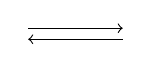
\begin{tikzpicture}
            \draw[->](0,0.07)--(1.2,0.07);
                    \draw[<-](0,-0.07)--(1.2,-0.07);
        \end{tikzpicture}  
        \chemfig{R-CH(-[270]NH_3^+)-COO^{-}} 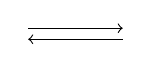
\begin{tikzpicture}
            \draw[->](0,0.07)--(1.2,0.07);
                    \draw[<-](0,-0.07)--(1.2,-0.07);
        \end{tikzpicture} \chemfig{R-CH(-[270]NH_3^+)-COO^{-}}
    \end{figure}
    \underline{        }       \underline{          }       \underline{        }\\
    \item ニンヒドリン溶液と温めると\underline{     }~〜~\underline{     }に呈色(\underline{        }反応).\\
    \item カルボキシ基があるので,アルコールと反応して\underline{        }化される.\\
    \item カルボキシ基があるので,アルコールと反応して\underline{        }化される.\\[1cm]
    \ce{R1-CH(NH2)-COOH + HO-R2 ->} \\[1cm]
    \item アミノ基が無水酢酸と反応して\underline{        }化される.\\[1cm]
    \ce{R1-CH(NH2)-COOH + (CH3CO)2O ->} \\[1cm]
        \item アミノ酸同士で分子間脱水して\underline{        }をつくる.\\[1cm]
    \ce{H2N-CH(R1)-COOH + H2N-CH(R_2)COOH ->} \\[1cm]
\end{itemize}
\newpage
\ascboxA{\textbf{タンパク質}}
\begin{itemize}
    \item 複数の$\alpha$-アミノ酸が\underline{       }結合でくっついた分子を\underline{         }という.
    \item タンパク質の正体はポリペプチドから成る.要するに,タンパク質は$\alpha$-アミノ酸からなる高分子化合物.
\end{itemize}
 \\
\ascboxA{\textbf{タンパク質の性質}}
\begin{itemize}
    \item \textbf{変性}\\
    熱・酸・塩基・重金属イオンによってタンパク質の立体構造が変化し,沈殿や凝固が起こること.この反応は不可逆的である.(例:肉を焼くと色が変わって固くなる)\\
    \item  \textbf{ビウレット反応(トリペプチド以上の検出)}\\
    ペプチド結合が\underline{   }個以上あるとき,水酸化ナトリウムと硫酸銅(II)水溶液を加えると\\[10pt]\underline{      }色を示す.\\
    \item  \textbf{キサントプロテイン反応(ベンゼン環の検出)}\\[10pt]
    \underline{            }を含むアミノ酸に濃硫酸を加えて加熱すると\underline{     }色を示す.\\
    \item  \textbf{ニンヒドリン反応(アミノ酸orタンパク質中のアミノ基の検出)}\\
    ニンヒドリン溶液を加えて加熱すると,\uwave{アミノ酸orタンパク質中のアミノ基}に反応して赤紫〜青紫色を示す.\\
    \item  \textbf{硫黄の検出反応}\\
    硫黄を含むアミノ酸に水酸化ナトリウム水溶液を加えて加熱した後,鉛(II)の塩を入れる\\[10pt]と\ce{PbS}の\underline{    }色沈殿を生じる.\\
    \item \textbf{ 窒素の検出反応}\\
    水酸化ナトリウム水溶液を加えて加熱した後,赤色リトマス紙を近づけると\underline{     }色になる.
\end{itemize}
\newpage
\begin{que}
    次の文中に当てはまる語や構造式を記せ.
    \begin{itemize}
        \item [(1)]タンパク質の加水分解で得られるアミノ酸はすべて\fbox{A}で,約20種類ある.アミノ酸を検出するには,\fbox{B}溶液により\fbox{C}色を呈することを確認すればよい.\\
        \item [(2)]アミノ酸は両性を示し,酸とも塩基とも反応する.一般に,アミノ酸\ce{R-CH(NH2)-COOH}は酸性溶液中では構造式\fbox{D}で表される\fbox{E}イオンに,中性付近では構造式\fbox{F}で表される\fbox{G}イオンに,塩基性溶液中では構造式\fbox{H}で表される\fbox{I}イオンになっている.\\
    \item[(3)]タンパク質は多数の\fbox{J}が\fbox{K}結合でつながった構造を持ち,水溶液に水酸化ナトリウムと硫酸銅(II)を加えると\fbox{L}色を呈することで確認できる.この反応を\fbox{M}反応という.
    \end{itemize}
\end{que}
\newpage
\begin{que}
次の文中に適切な数値,記号,語句を入れよ.また,[   ]には適当なアミノ酸の名称を下の語群からすべて選んで入れよ.\\

 タンパク質を加水分解すると,約\fbox{A}種類の\fbox{B}が得られる.このアミノ酸は一般式\ce{R-CH(NH2)-COOH}で表され,[ あ ]以外は不斉炭素原子を持つ.\\
 Rが\ce{CH3}のアミノ酸を\fbox{C}といい,これは多くのタンパク質に含まれている.また,Rの部分に\ce{-OH}を持つものには[ い ],ベンゼン環を持つものには[ う ],\ce{-NH2}を持つものには[ え ],\ce{-COOH}を持つものには[ お ]などがある.\\[5pt]
\textbf{語群}\\
グリシン,アラニン,フェニルアラニン,システイン,セリン,リシン,メチオニン,チロシン,グルタミン酸
\end{que}
\end{document}